\documentclass[a4paper]{article}
\usepackage[utf8]{inputenc}
\usepackage[russian]{babel}
\usepackage[T2]{fontenc}
\usepackage[warn]{mathtext}
\usepackage{graphicx}
\usepackage{floatflt}
\usepackage[left=30mm, top=20mm, right=20mm, bottom=20mm, footskip=10mm]{geometry}


\graphicspath{ {images/} }
\usepackage{multicol}
\setlength{\columnsep}{2cm}


\begin{document}

\begin{titlepage}
	\centering
	\vspace{5cm}
	{\scshape\LARGE Московский физико-технический институт \par}
	\vspace{4cm}
	{\scshape\Large Лабораторная работа \par}
	\vspace{1cm}
	{\huge\bfseries Определение вязкости жидкости по скорости истечения через капилляр \par}
	\vspace{1cm}
	\vfill
\begin{flushright}
	{\large выполнила студентка 653 группы ФФКЭ}\par
	\vspace{0.3cm}
	{\LARGE Карпова Татьяна}
\end{flushright}
	

	\vfill

% Bottom of the page
	Долгопрудный, 2017 г.
\end{titlepage}

\section{Цель работы}

\begin{enumerate}
    \item определение вязкости воды по измерению объёма жидкости, протёкшей через капилляр
    \item определение вязкости других жидкостей путём сравнения скорости их перетекания со скоростью перетекания воды
\end{enumerate}

\section{В работе используются}
\begin{itemize}
    \item сосуд Мариотта
    \item капиллярная трубка
    \item мензурка
    \item секундомер
    \item стакан
    \item микроскоп на стойке
\end{itemize}

\section{Измерение вязкости воды}
\subsection{Теоретические положения}
Формула Пуазейля для расхода жидкости через сечение трубки:
\begin{center}
$Q = \pi \frac{P_1-P_2}{8 \eta l} R^4$
\end{center}

Число Рейнольдса:
\begin{center}
$Re = \frac{v R \rho}{\eta} = \frac{2\frac{\rho v^2}{2}}{\eta \frac{v}{R}}$
\end{center}
Согласно уравнению Бернулли, 
\begin{center}
$\frac{\rho v^2}{2} = P_0 - P$
\end{center}

В гладких трубах круглого сечения переход от ламинарного движения к турбулентному происходит при $Re \approx 1000$.

Ламинарное движение жидкости при переходе ее из широкого сосуда в капилляр устанавливается не сразу, а после того, как она пройдет расстояние $a$
\begin{center}
$a = 0,2R * Re$
\end{center}

\subsection{Экспериментальная установка}

\begin{figure}[h]
    \centering
    \includegraphics[width=7cm]{setup1.PNG}
    \caption{Схема установки для определения вязкости воды}
    \label{fig:vac}
\end{figure}

Установка для измерения вязкости воды изображена на рис. 1.
Вода заполняет сосуд Мариотта и вытекает через калиброванную капиллярную трубку, укрепленную в нижней части его боковой стенки. Сосуд Мариотта позволяет поддерживать постоянным перепад давления $P_1 - P_2$ на концах капилляра, несмотря на то, что уровень жидкости при ее вытекании понижается. Это достигается с помощью трубки В, открытой в атмосферу и проходящей через пробку, герметично закрывающую сосуд. \par
Величина перепада давления $P_1 - P_2$ определяется высотой столба воды $h$ между осью капиллярной трубки А и нижним концом вертикальной трубки В. Высота столба измеряется с помощью микроскопа М, укрепленного на вертикально перемещающемся плунжере. Смещение плунжера определяется по миллиметровой шкале, снабженной нониусом. Объем вытекшей жидкости измеряется мензуркой П. Время истечения определяется по секундомеру. Длина капиллярной трубки измеряется миллиметровой линейкой, диаметр ---
 микроскопом МИР.


\subsection{Ход работы}
\begin{enumerate}
    \item С помощь микроскопа определим радиус трубки: $R = 0,475$ мм. \par
    С помощью миллиметровой линейки определим длину капилляра: $l = 12$ см
    \item Убедимся, что расход воды при одинаковой величине $h$ не зависит от уровня жидкости. При $h = 39$ см объём 20 см$^3$ вытек из сосуда сначала за 410 с, затем за 412 с. Условие выполняется.
    \item Перепад давлений $\triangle P = P_1 - P_2$ между концами капилляра, выраженный в миллиметрах водяного столба, не равен $h$, а содержит поправку $\triangle h$, обусловленную силами поверхностного натяжения. Чтобы её определить, будем опускть трубку В до тех пор, пока вода не перестанет вытекать из капилляра, это значит, что Это значит, что давление столба воды $\triangle h$ между осью капилляра и нижним торцом трубки В уравновесилось силами поверхностного натяжения пузырька воздуха, возникшего на конце трубки В, и капли жидкости на конце трубки С.
    \begin{center}
    $\triangle h = 9,5$ мм
    \end{center}
    \item Измерим расход воды при нескольких значениях $h$. Результаты занесём в таблицу 1. По формуле для числа Рейнольдса $Re = \frac{vR \pho}{\eta} = \frac{QR \rho}{S \eta} = \frac{V\rho}{\pi R \eta t}$ удостоверимся, что в каждом из опытов в капилляре устанавливается ламинарное течение. По формуле $a = 0,2R * Re$ оценим длину участка капилляра, по прохождении которого устанавливается ламинарное течение. Результаты также занесём в таблицу 1.
    
    \begin{table}[h]
    \centering
    \begin{center}
    \caption{Зависимость расхода воды от перепада давлений в сосуде Мариотта}
    \end{center}
    \vspace{0.1cm}
    \label{tab:my_label}
    \begin{tabular}{ |p{1.5cm}|p{1.5cm}|p{1.5cm}|p{1.5cm}|p{1.5cm}|  }
    \hline
     h, мм & t, c & Q, см$^3$/c & Re & a, мм\\
    \hline 
     41,4 & 392 & 0,0510 & 74,62 & 3,73 \\
     50,5 & 297 & 0,0673 & 98,49 & 4,92 \\
     63,5 & 225 & 0,0889 & 130,00 & 6,50 \\
     74,5 & 189 & 0,1058 & 154,77 & 7,74 \\
    \hline
    \end{tabular}
    \end{table}
    
    \item Представим полученные результаты на графике $Q(h)$ - рис. 2. По расчётам, представленным в п. 3.4, ламинарное течение устанавливается практически сразу же во всех опытах, поэтому наблюдаем чёткую линейную зависимость. Формула Пуазейля для расхода:
    \begin{center}
    $Q = \pi \frac{P_1-P_2}{8 \eta l} R^4 = \pi \frac{(h - \triangle h)\rho g}{8 \eta l} R^4$;
    \end{center}
    по формуле видно, что на графике $\triangle h$ отсекается аппроксимирующей прямой при $Q = 0$ и $\triangle h = 10$ мм. Определённое экспериментально значение $\triangle h = 9,5$ мм примерно ему равно.
    
    \begin{figure}[t]
    \centering
    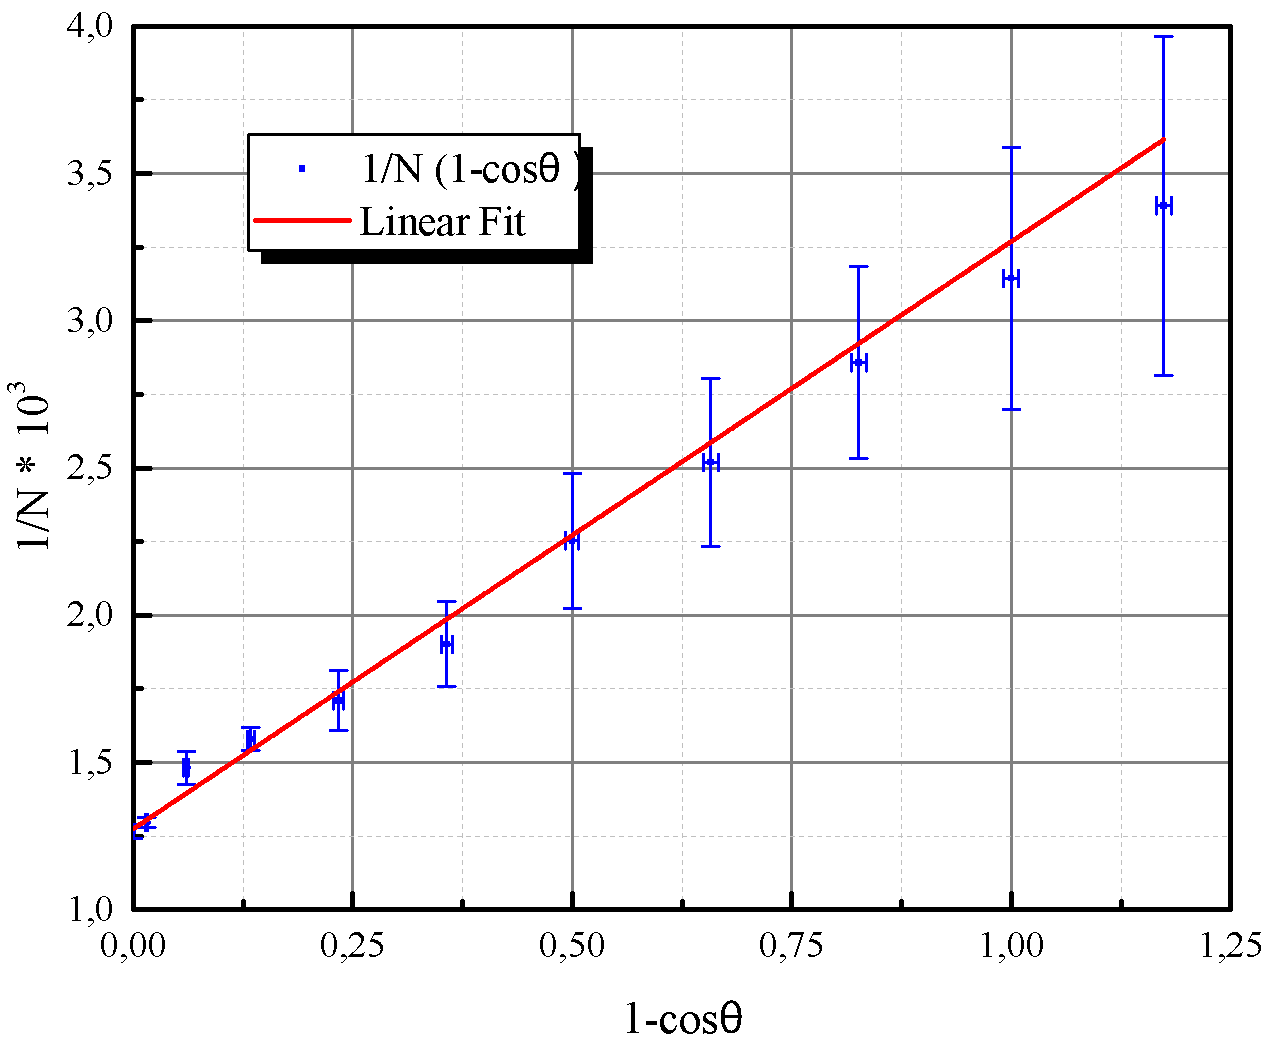
\includegraphics[width=\textwidth]{graph1.PNG}
    \caption{График зависимости расхода воды от высоты столба воды в сосуде}
    \label{fig:vac}
    \end{figure}
    
    По углу наклона прямой определим величину $\eta$
    \begin{center}
    $\eta = \frac{\pi R^4 \rho g}{8 l Q'(h)} = 0.00894$ П
    \end{center}
    
    Оценим погрешность определения вязкости по формуле
    \begin{center}
    $\sigma \eta = \eta \sqrt{(\frac{\sigma h}{h})^2 + 4^2(\frac{\sigma R}{R})^2 + (\frac{\sigma l}{l})^2} = 0,000616$ П
    \end{center}
    
    Для воды температуры 25$^{\circ} $C значение вязкости $\eta = 0,00891$ П. \par
    С учётом погрешности величина, определённая экспериментально, и величина из таблицы (tehtab.ru)  равны.
    
    \begin{center}
    \fbox
    {$\eta_t_h = 0,00891$ П \hspace{1cm} $\eta_e_x = 0,00894 \pm 0,0006$ П}
    \end{center}

    
\end{enumerate}

    \section{Измерение вязкости водного раствора глицерина вискозиметром Оствальда}
    
    \subsection{Теоретические положения}
    
    Заменяя в формуле Пуазейля $Q_v$ на $-dV/dt$ и $P_1 - P_2$ на $\rho h(v) g$, получим 
    \begin{center}
    $-\frac{dV}{dt} = \frac{\pi R^4}{8l}\frac{h(V)\rho g}{\eta}$, или $-\frac{8l}{\pi R^4}\frac{dV}{h(V)} = \frac{\rho g}{\eta}dt$
    \end{center}
    Интегрируя от $V = V_0$ до $V = V_1$ и от $t = 0$ до $t = t_1$ получим, что
    \begin{center}
    $\frac{\rho_1}{\eta_1}t_1 = \frac{\rho_2}{\eta_2}t_2 = \frac{\rho_3}{\eta_3}t_3 = ...$
    \end{center}
    
    Проведя опыты с водой, а затем с исследуемой жидкостью, получим
    \begin{center}
    $\eta_x = \eta_0\frac{\rho_x}{\rho_0}\frac{t_x}{t_0}$
    \end{center}
    
    \subsection{Экспериментальная установка}
    
    \begin{figure}[t]
    \centering
    \includegraphics[width=30mm]{setup2.jpg}
    \caption{Вискозиметр Оствальда}
    \label{fig:vac}
    \end{figure}
    
    Вискозиметр Оствальда представляет собой стеклянную трубку с расширением наверху. С помощью резиновой груши, подсоединенной  резиновой трубкой к отверстию 1, засасывают воду так, чтобы ее мениск поднялся несколько выше метки М1. Сняв грушу с трубки и удерживая вискозиметр в вертикальном положении, дают возможность воде свободно протекать через шарик 4. Когда мениск проходит метку М1, включают секундомер, и выключают его, когда мениск проходит метку М2. Таким образом измеряют время t0, за которое объем воды V , заключенный между метками, протекает через капилляр. В вискозиметре Оствальда диаметр капилляра и перепад давления на нем подобраны так, что течение жидкости в капилляре всегда является ламинарным.
    
    \subsection{Ход работы}
\begin{enumerate}
    \item Определим время перетекания воды между метками. Измерения проводим 10 раз, затем усредняем значения. Те же измерения проводим с 10-, 20-, 30-\% растворами глицерина. Результаты измерений занесём в таблицу 2.

    \begin{table}[h]
    \centering
    \begin{center}
    \caption{Время протекания жидкостей между метками}
    \end{center}
    \vspace{0.05cm}
    \label{tab:my_label}
    \begin{tabular}{ |p{3cm}|p{3cm}|p{3cm}|p{3cm}| }
    \hline
     Вода, t, c & Глицерин 10\%, t, c & Глицерин 20\%. t, c & Глицерин 30\%, t, c \\ 
    \hline
    $\rho$ = 997,13 кг/м$^3$ & $\rho$ = 1019,2 кг/м$^3$ & $\rho$ = 1041,5 кг/м$^3$ & $\rho$ = 1064,6 кг/м$^3$\\
    \hline
    5,88 & 8,41 & 12,31 & 13,10\\
    5,95 & 8,41 & 12,45 & 13,04\\
    5,97 & 8,47 & 12,31 & 13,05\\
    5,91 & 8,48 & 12,34 & 13,00\\
    5,94 & 8,51 & 12,35 & 13,05\\
    6,00 & 8,51 & 12,28 & 13,01\\
    5,93 & 8,59 & 12,34 & 13,01\\
    5,97 & 8,51 & 12,34 & 13,17\\
    5,97 & 8,54 & 12,31 & 13,01\\
    5,94 & 8,36 & 12,35 & 13,08\\
    
    \hline
    \hline
    
    $\bar t = 5,95$ с & $\bar t = 8,48$ с & $\bar t = 12,34$ с & $\bar t = 13,06$ с \\
    \hline
    $\sigma_t = 0,01$ c & $\sigma_t = 0,02$ c & $\sigma_t = 0,01$ c & $\sigma_t = 0,02$ c \\
    \hline
    \end{tabular}
    \end{table}  
    
    \item По формуле из 4.1 определим вязкости растворов глицерина различной концентрации. 
    \begin{center}
    $\eta_x = \eta_0\frac{\rho_x}{\rho_0}\frac{t_x}{t_0}$
    \end{center}
    Погрешность измерений оценим по формуле
    \begin{center}
     $\sigma \eta_x = \eta_x \sqrt{(\frac{\sigma \eta_0}{\eta_0})^2 + 4^2(\frac{\sigma t_x}{t_x})^2 + (\frac{\sigma t_0}{t_0})^2}$
    \end{center}
    
    \begin{center}
    $\eta_1_0 = 1,122 \pm 0,088$ сП\\
    $\eta_2_0 = 1,669 \pm 0,13$ сП\\
    $\eta_3_0 = 1,805 \pm 0,14$ сП\\
    \end{center}
    
    Сравним полученные нами результаты с табличными значениями (c сайта chem21.info)
    
    \begin{figure}[h]
    \centering
    \includegraphics[width=70mm]{table.png}
    \label{fig:vac}
    \end{figure}
    
    В пределах погрешности сходятся результаты для 10- и 20-\% растворов, для 30\% раствора различие составляет 0,3 сП.

\end{enumerate}

\section{Вывод}
 В ходе работы были разными способами определены вязкости разных жидкостей: определена вязкость воды по измерению объёма жидкости, прошедшей через капилляр, и определены вязкости водных растворов глицерина разных концентраций  с помощью вискозиметра Оствальда.
 \begin{enumerate}
     \item Значение вязкости воды, полученное первым способом, совпадает с табличным практически полностью (различается третий значащий знак)
     \begin{center}
    $\eta_t_h = 0,00891$ П \hspace{1cm}\\ $\eta_e_x = 0,00894 \pm 0,0006$ П
    \end{center}
     \item Почти все результаты (2 из 3), полученные во второй части работы, совпадают с табличными в пределах погрешности.\\
     \begin{center}
     $\eta_1_0_e = 1,122 \pm 0,088$ сП \hspace{1cm} $\eta_1_0_t = 1,153$ сП\\
    $\eta_2_0_e = 1,669 \pm 0,13$ сП \hspace{1cm} $\eta_2_0_t = 1,542$ сП\\
    $\eta_3_0_e = 1,805 \pm 0,14$ сП \hspace{1cm} $\eta_3_0_t = 2,157$ сП\\
    \end{center}
     Последний эксперимент (30\% раствор глицерина) проводился последним, лаборанты сами выдали нам раствор, но на нём не была указана концентрация. Возможно, это был раствор с меньшей концентрацией глицерина, примерно 25\% (даже проанализировав данные о времени протекания раствора между отметками, можно сказать, что он меньше ожидаемых). Для чистоты эксперимента оптимально было бы провести опыт с 30\% глицерином ещё раз и заново проанализировать результаты.
 \end{enumerate}

\end{document}
